\documentclass{../local}

\title{\textbf{Scriptie - Actieve Evacuatie Navigatie door middel van Wireless Sensor Networks}}
\author{\\
		Hogeschool Utrecht\\
		\\
		Roy Scheefhals - 1563303}

\begin{document}

\begin{titlepage}
\begin{center}

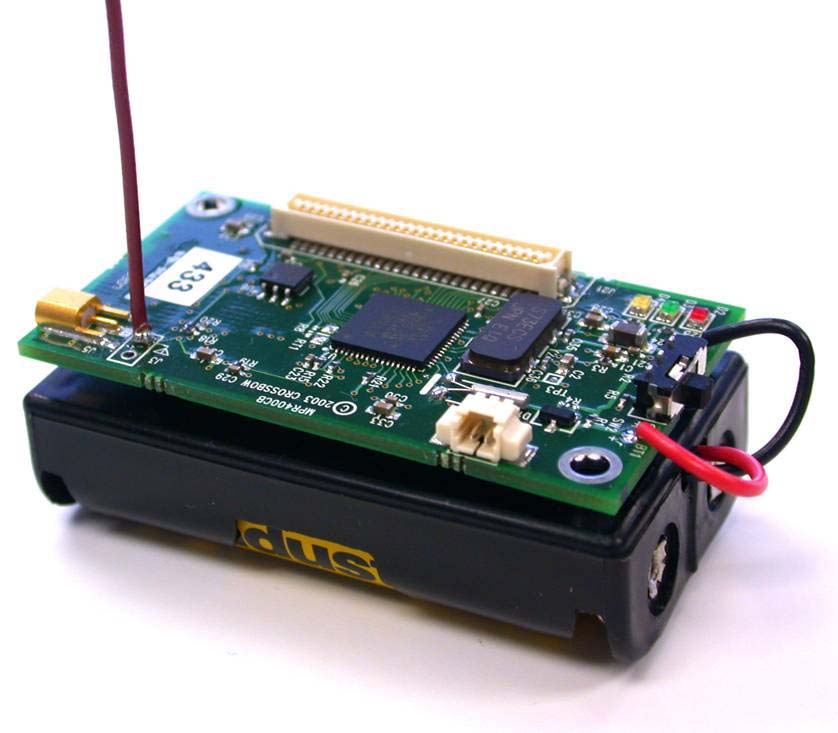
\includegraphics[width=0.6\textwidth]{../images/mica2}~\\[1cm]

{ \huge \bfseries Scriptie: Actieve Evacuatie Navigatie d.m.v. Wireless Sensor Networks\\[0.4cm] }
\hrule
\hspace{0pt} 
\vspace{\fill}

\begin{minipage}{0.4\textwidth}
\begin{flushleft} \large
\emph{Afstudeerder:}\\
Roy \textsc{Scheefhals}\\
\emph{Hogeschool Utrecht}\\
Studentnummer: 1563303\\
\end{flushleft}
\end{minipage}
\begin{minipage}{0.4\textwidth}
\begin{flushright} \large
\emph{Bedrijfsbegeleider:} \\
Martin \textsc{Klomp}\\
\emph{Alten PTS}
\end{flushright}
\end{minipage}

\end{center}
\today
\end{titlepage}

\renewcommand{\thesection}{\Roman{section}}
\newpage\pagenumbering{roman}

\section{Termen en Afkortingen}
\subfile{Termen}

\newpage\pagenumbering{arabic}
\renewcommand{\thesection}{\arabic{section}}
\setlength{\cftbeforetoctitleskip}{-3em}
\tableofcontents

\clearpage

\chapter{Inleiding}
\subfile{Inleiding}

\chapter{Context Project} 
\subfile{Achtergrond}

\chapter{Project Definitie}
\subfile{Opdracht}

%TODO: gebruikte tools
%doxygen
%latex? 

\chapter{Gemaakte Keuzes}
\subfile{Keuzes}

\chapter{Ontwerpen}
\subfile{Ontwerpen}

\chapter{Implementatie}
\subfile{Implementatie}

\chapter{Conclusie \& Discussie}
\subfile{Conclusie}

\chapter{Aanbevelingen}
\subfile{Aanbevelingen}

\bibliographystyle{apalike2}
\bibliography{mybib}

\subfile{Bijlagen}


\end{document}
